%%----------------------------------------------------------------------------
%% Presentatie HoGent Bedrijf en Organisatie
%%----------------------------------------------------------------------------
%% Auteur: Bert Van Vreckem [bert.vanvreckem@hogent.be]

\documentclass{beamer}

%==============================================================================
% Aanloop
%==============================================================================

%---------- Packages ----------------------------------------------------------
\usepackage{etex}
\usepackage{graphicx,multicol}
\usepackage{comment,enumerate,hyperref}
\usepackage{amsmath,amsfonts,amssymb}
\usepackage{tikz}
\usepackage[dutch]{babel}
\usepackage[utf8]{inputenc}
\usepackage{multirow}
\usepackage{eurosym}
\usepackage{listings}
\usepackage[T1]{fontenc}
\usepackage{lmodern}
\usepackage{textcomp}
\usepackage{framed}
\usepackage{wrapfig}
\usepackage{pgf-pie}
\usepackage{pgfplots}
\usepackage{booktabs}
\usepackage{pgfplotstable}
\usepackage{changepage}

%---------- Configuratie ------------------------------------------------------

\usetikzlibrary{arrows,shapes,backgrounds,positioning,shadows}
\usetikzlibrary{pgfplots.statistics}

\usetheme{hogent}
\setbeameroption{show notes}

%---------- Command-definitions -----------------------------------------------

\newcommand{\tabitem}{~~\llap{\textbullet}~~}
\renewcommand{\arraystretch}{1.2}

%---------- Document metadata ------------------------------------------

\title[Bivariate Analysis]{Research Techniques\\5. Bivariate Analysis}
\author{Wim Goedertier, Jens Buyse, Bert {Van Vreckem}, Wim {De Bruyn}}
\date{AY 2017-2018}

\begin{document}

%---------- Front matter ------------------------------------------------------

% Dia met het HoGent logo
\HoGentLogo

% Titeldia met faculteitslogo
\titleframe

%---------- Inhoud ------------------------------------------------------------

\begin{frame}
  \frametitle{What's on the menu today?}

  \tableofcontents
\end{frame}

\section{Recap: Plotting variables / Presenting data}
\sectionframelogo{}

\begin{frame}
  \frametitle{Example case: survey college restaurant visitors}

  \begin{figure}
    \centering
    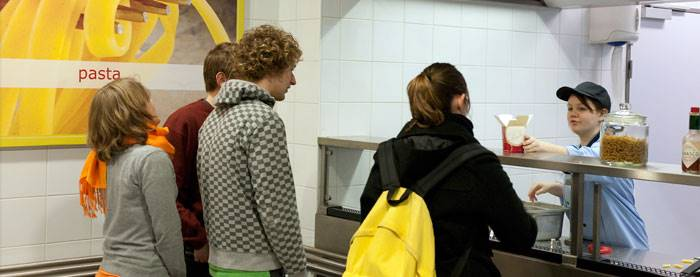
\includegraphics[width=0.8\textwidth] {img/students.jpg}
    \label{fig:students}
  \end{figure}

  \begin{itemize}
    \item What's the number of days per week that people go to the restaurant? (1 variable)
    \item Is there a difference in spending between students and staff? (comparing nominal vs. quantitative variable)
%    \item Is there a link between the number of visits and the total amount spent?
  \end{itemize}

  R Code: see \texttt{syllabus/data/catering\_college.R}

\end{frame}

\begin{frame}
  \frametitle{What's the number of days per week that people go to the restaurant? (1 variable)}
  
  \begin{columns}
    \begin{column}{0.5\textwidth}
      \begin{table}[h]
        \begin{tabular}{|l|l|}
        	\hline
        	{\textbf{Statistic}} & \textbf{Value} \\ \hline
        	Mean                 & 2.96           \\ \hline
        	Median               & 3              \\ \hline
        	Mode                 & 2              \\ \hline
        	Stdev                & 1.484          \\ \hline
        	Variance             & 2.202          \\ \hline
        	Range                & 4              \\ \hline
        	$Q_{1}$              & 2              \\ \hline
        	$Q_{2}$              & 3              \\ \hline
        	$Q_{3}$              & 5              \\ \hline
        \end{tabular}
      \end{table}
    \end{column}
    \begin{column}{0.5\textwidth}

      \begin{figure}
        \centering
        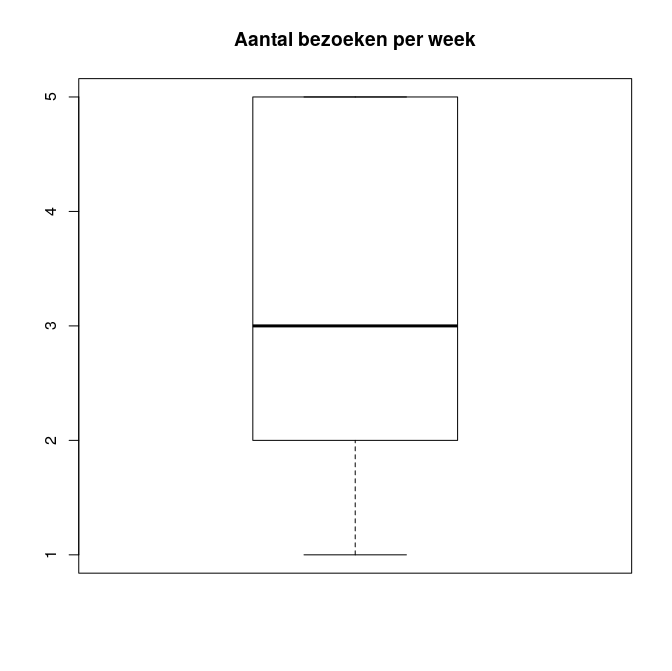
\includegraphics[width=1.00\textwidth]{img/2var-boxplot-aantalbezoeken}
      \end{figure}

    \end{column}
  \end{columns}
\end{frame}

\begin{frame}
  \frametitle{What's the number of days per week that people go to the restaurant? (1 variable)}
  \begin{columns}
    
    \begin{column}{0.5\textwidth}
      \begin{figure}
        \centering
        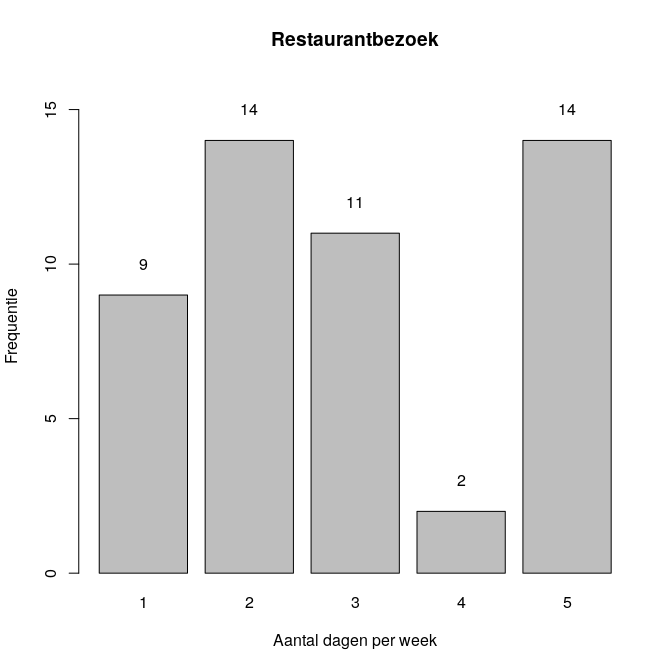
\includegraphics[width=1.00\textwidth]{img/2var-barplot-aantalbezoeken}
      \end{figure}
    \end{column}
  
    \begin{column}{0.5\textwidth}
      \begin{figure}
        \centering
        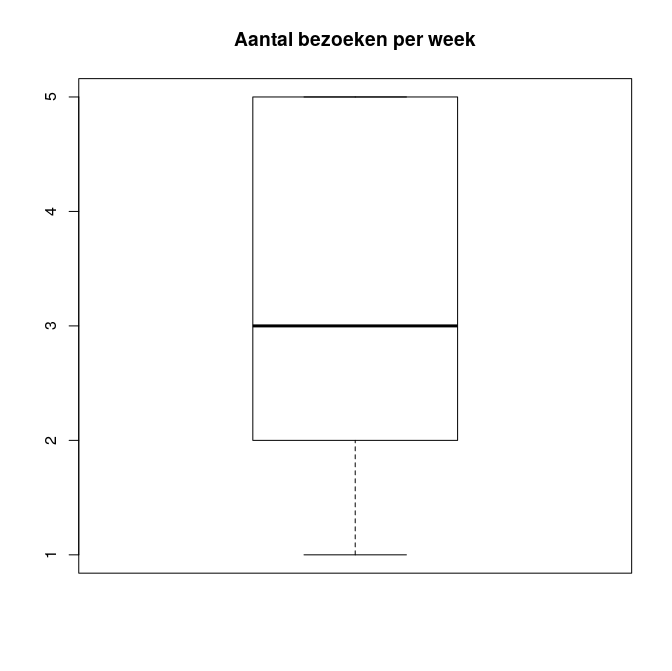
\includegraphics[width=1.00\textwidth]{img/2var-boxplot-aantalbezoeken}
      \end{figure}
    \end{column}
  
  \end{columns}
\end{frame}

\begin{frame}
  \frametitle{Is there a difference in spending between students and staff? (comparing nominal vs. quantitative variable)}
  \begin{itemize}
    \item \alert<1>{Bar chart} (of averages per category)
    \item \alert<2>{Boxplot}
  \end{itemize}

  \begin{figure}
    \centering
    \only<1>{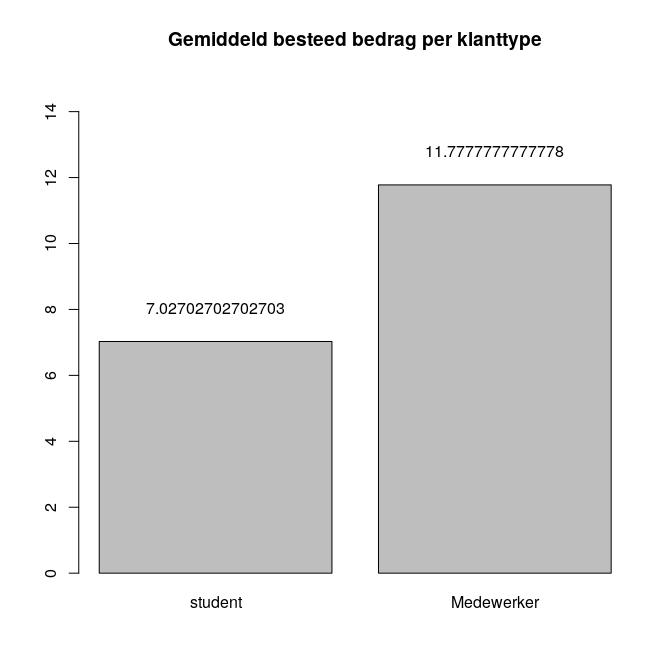
\includegraphics[width=0.5\textwidth]{img/2var-barplot-gemiddeld-bedrag}}
    \only<2>{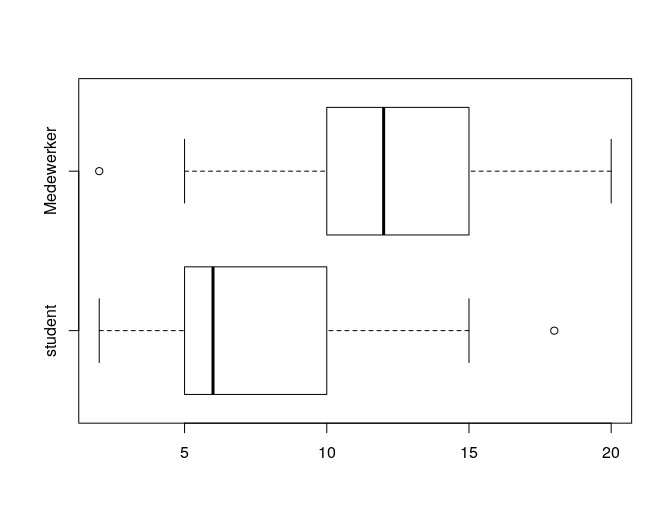
\includegraphics[width=0.7\textwidth]{img/2var-boxplot-klanttype-bedrag}}
  \end{figure}

  \only<1>{\textbf{Remark!} Not sufficient to prove a significant difference!}
\end{frame}

\section{Contingency tables and Cramér's V}
\sectionframelogo{}

\begin{frame}
  \frametitle{Contingency tables}
  (also: cross tabulation, crosstab, Dutch: \emph{kruistabel})
  \vfill
  This is used for \textbf{categorical data},\\
  i.e. to compare 2 qualitative (nominal or ordinal) variables.
  \vfill
  Is there a difference in the appreciation of the basic product range between men and women?
  \begin{table}[h]
    \begin{tabular}{l||l|l||l}
                   & Women & Men & Total \\ \hline\hline
      Good         & 9     & 8   & 17    \\
      Sufficient   & 8     & 10  & 18    \\
      Insufficient & 5     & 5   & 10    \\
      Bad          & 0     & 4   & 4     \\ \hline\hline
      Total        & 22    & 27  & 49
    \end{tabular}
  \end{table}
\end{frame}

\begin{frame}
  \frametitle{Contingency tables}
  
  Estimating association between two nominal variables: $\chi^2$ (chi squared)
  
  \[ \chi^2 = \sum_i \frac{(a_i - e_i)^2}{e_i} \]
  
  \begin{itemize}
    \item $i$ iterates over all cells in the table
    \item $a$ is the observed value
    \item $e$ is the expected value if there is no difference between categories being compared
  \end{itemize}
  
\end{frame}

\begin{frame}
  \frametitle{Contingency tables: percentages}
  Is there a difference in the appreciation of the basic product range between men and women?
  \begin{adjustwidth}{-1.5em}{-1.5em}
    \begin{table}[h] \centering
      \begin{tabular}{@{}rrrrrrr@{}}
        \toprule
                     & Women &  Men & Total & Women \% &   Men\% &   Total \\ \midrule
                Good &   $9$ &  $8$ &  $17$ &   $41$\% &  $30$\% &  $35$\% \\
          Sufficient &   $8$ & $10$ &  $18$ &   $36$\% &  $37$\% &  $37$\% \\
        Insufficient &   $5$ &  $5$ &  $10$ &   $23$\% &  $18$\% &  $20$\% \\
                 Bad &   $0$ &  $4$ &   $4$ &    $0$\% &  $15$\% &   $8$\% \\
               Total &  $22$ & $27$ &  $49$ &  $100$\% & $100$\% & $100$\% \\ \bottomrule
      \end{tabular}
    \end{table}
  \end{adjustwidth}
  \vfill
  See also codingexamples/6-bivariate-analysis-CramersV.xlsx
\end{frame}

\begin{frame}
  \frametitle{Contingency tables: differences}
  Is there a difference in the appreciation of the basic product range between men and women?
  \begin{adjustwidth}{-1.5em}{-1.5em}
    \begin{table}[h] \centering
      \begin{tabular}{@{}rrrrrrr@{}}
        \toprule
                     &                       Women &                          Men & Total & Women \% &   Men\% &   Total \\ \midrule
                Good &  $9 -\textcolor{red}{7.63}$ &  $8 - \textcolor{red}{9.36}$ &  $17$ &   $41$\% &  $30$\% &  $35$\% \\
          Sufficient & $8 - \textcolor{red}{8.08}$ & $10 - \textcolor{red}{9.91}$ &  $18$ &   $36$\% &  $37$\% &  $37$\% \\
        InSufficient & $5 - \textcolor{red}{4.48}$ &  $5 - \textcolor{red}{5.51}$ &  $10$ &   $23$\% &  $18$\% &  $20$\% \\
                 Bad & $0 - \textcolor{red}{1.79}$ &  $4 - \textcolor{red}{2.20}$ &   $4$ &    $0$\% &  $15$\% &   $8$\% \\
               Total &                        $22$ &                         $27$ &  $49$ &  $100$\% & $100$\% & $100$\% \\ \bottomrule
      \end{tabular}
    \end{table}
  \end{adjustwidth}
\end{frame}

\begin{frame}
  \frametitle{Contingency tables: squared difference, normalisation}
  Is there a difference in the appreciation of the basic product range between men and women?
  \begin{table}[h] \centering
    \begin{tabular}{@{}rrrrrrr@{}}
      \toprule
                   &                   Women &                     Men & Total & Women \% &   Men\% &   Total \\ \midrule
              Good & $\textcolor{blue}{0.2}$ & $\textcolor{blue}{0.2}$ &  $17$ &   $41$\% &  $30$\% &  $35$\% \\
        Sufficient &   $\textcolor{blue}{0}$ &   $\textcolor{blue}{0}$ &  $18$ &   $36$\% &  $37$\% &  $37$\% \\
      InSufficient & $\textcolor{blue}{0.1}$ &   $\textcolor{blue}{0}$ &  $10$ &   $23$\% &  $18$\% &  $20$\% \\
               Bad & $\textcolor{blue}{1.8}$ & $\textcolor{blue}{1.5}$ &   $4$ &    $0$\% &  $15$\% &   $8$\% \\
             Total &                    $22$ &                    $27$ &  $49$ &  $100$\% & $100$\% & $100$\% \\ \bottomrule
    \end{tabular}
  \end{table}
  \[ \chi^{2} = 3.811, V= 0.279 \]
\end{frame}

\begin{frame}
  \frametitle{Cramér's V}
  \brightbox{\textcolor{HoGentAccent6}{Cramér's V} is a measure (between 0 and 1) that indicates how strong the association between two nominal variables is.}
  
  \[ V = \sqrt{\frac{\chi^2}{n \cdot \mathrm{min}(k - 1, l - 1)}} \]
  
  with $k$ and $l$ the number of categories for each variable
  
  \begin{table}[h] \centering
    \begin{tabular}{@{}rr@{}}
    	\toprule
    	 Value &            Interpretation \\ \midrule
    	   $0$ &            no association \\
    	 $0.1$ &          weak association \\
    	$0.25$ & fairly strong association \\
    	 $0.5$ &        strong association \\
    	$0.75$ &   very strong association \\
    	   $1$ &      complete association \\ \bottomrule
    \end{tabular}
  \end{table}
\end{frame}

\begin{frame}
  \frametitle{Example 2: link between gender and car brand preferences}
  \begin{table}[h] \centering
    \begin{tabular}{@{}rrrrrr@{}}
    	\toprule
    	      & Mercedes &  BMW & Porsche & Alfa Romeo & Total \\ \midrule
    	  Men &     $10$ & $10$ &    $20$ &       $20$ &  $60$ \\
    	Women &     $20$ &  $5$ &    $15$ &        $0$ &  $40$ \\
    	Total &     $30$ & $15$ &    $35$ &       $20$ & $100$ \\ \bottomrule
    \end{tabular}
  \end{table}

  It seems that car brands are not preferred equally by men and women.
  \[ \chi^{2} = 22.619 \]
  \[ V = \sqrt{\frac{22.169}{100 . (2-1)}}  = 0.476\]
\end{frame}

\begin{frame}
  \frametitle{Example 2: link between gender and car brand preferences}

  \begin{figure}
    \centering
    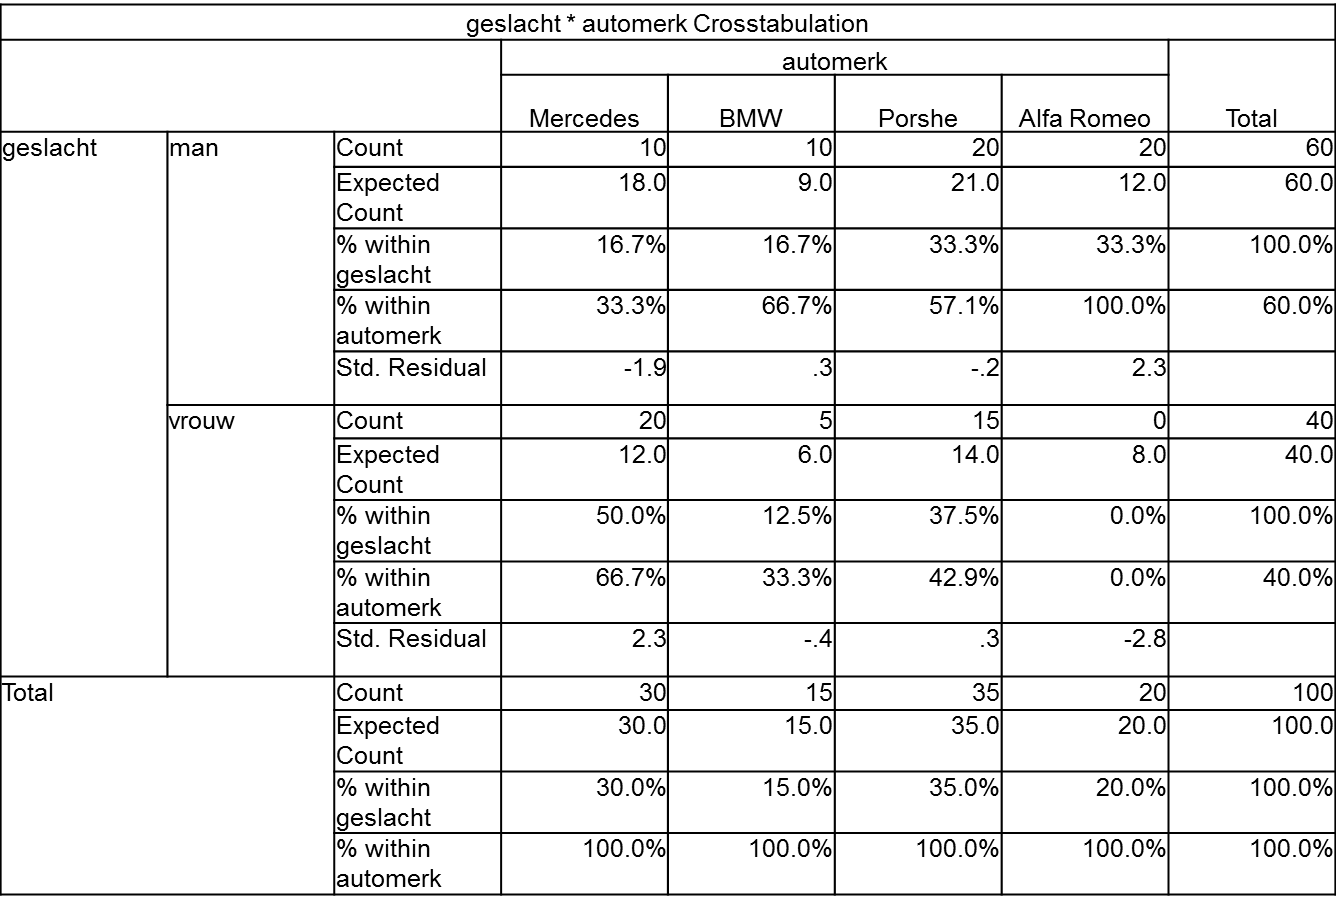
\includegraphics[width=1.00\textwidth]{img/les3-spssCars.png}
    \label{fig:les3-spssCars}
  \end{figure}

\end{frame}

\begin{frame}
  \frametitle{Visual representation of contingency tables}
  \framesubtitle{Mosaic plot}
  
  \begin{figure}
    \centering
    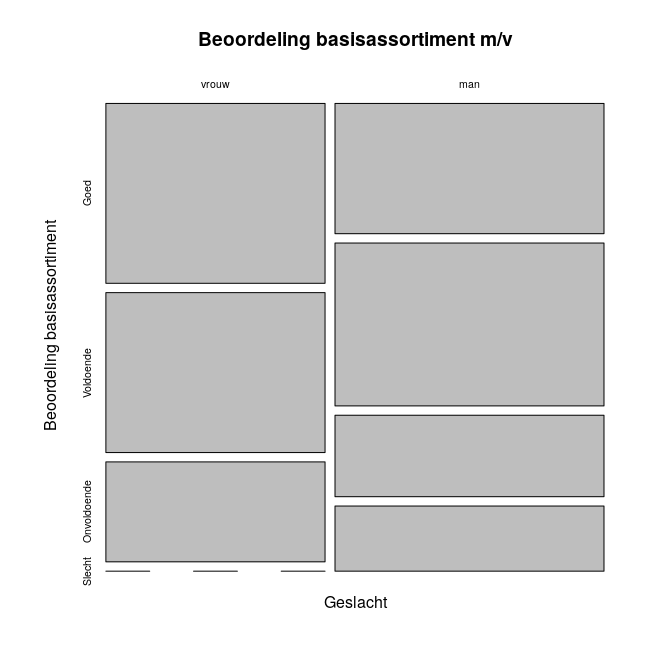
\includegraphics[width=0.80\textwidth]{img/2var-xtab-plot-waardering}
  \end{figure}
  
\end{frame}

\begin{frame}
  \frametitle{Visual representation of contingency tables}
  \framesubtitle{Clustered bar chart}

  \begin{figure}
    \centering
    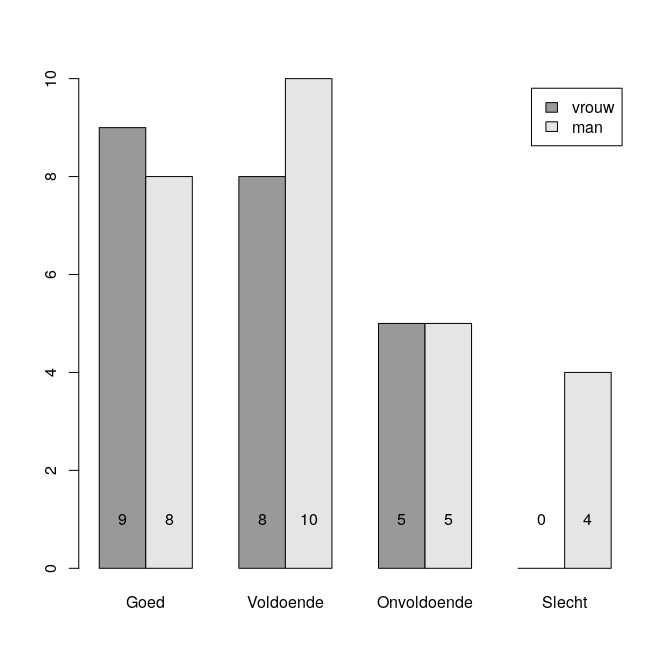
\includegraphics[width=0.80\textwidth]{img/2var-staafgrafiek-geclusterd}
  \end{figure}

\end{frame}

\begin{frame}
  \frametitle{Visual representation of contingency tables}
  \framesubtitle{Stacked percentage bar chart}
  
  \begin{figure}
    \centering
    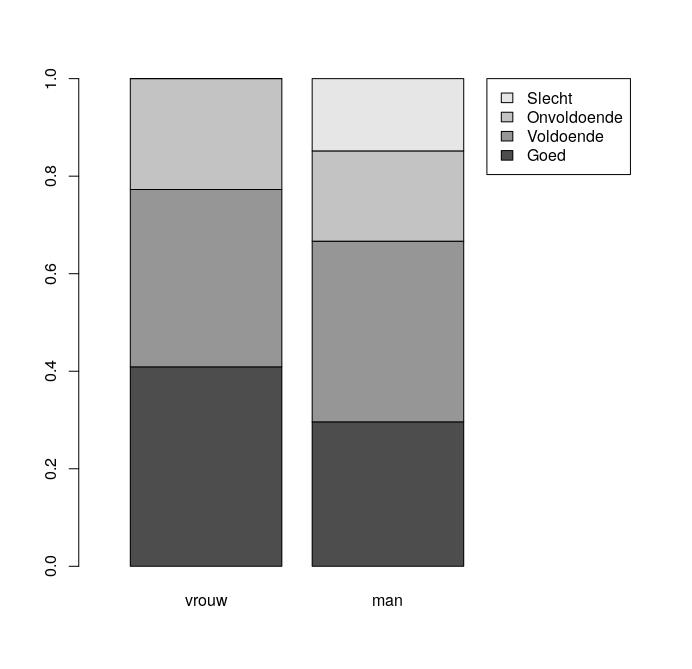
\includegraphics[width=0.80\textwidth]{img/2var-rependiagram-waardering-mv}
  \end{figure}

\end{frame}

\section{Linear Regression}
\sectionframelogo{}

\begin{frame}
  \frametitle{Linear Regression}
  
  \brightbox{\textcolor{HoGentAccent6}{Regression} is searching for a \textcolor{HoGentAccent6}{consistent} and \textcolor{HoGentAccent6}{systematic} association between variables.}
\vfill
  The association can be:
  \begin{enumerate}
    \item \textbf{Monotonous:} consistently increasing or consistently decreasing
    \item \textbf{Non-monotonous:} going up and down
  \end{enumerate}
\vfill
  The association can also be:
  \begin{enumerate}
    \item \textbf{Linear:} it can be describe by a line
    \item \textbf{Non-linear:} e.g. quadratic, logaritmic, ...
  \end{enumerate}
\end{frame}

\begin{frame}
  \frametitle{Linear regression}
  \centering
  \begin{tikzpicture}
    \begin{axis}[
        axis x line=middle,
        axis y line=middle,
        enlarge y limits=true,
        width=\textwidth, height=8cm,     % size of the image
        grid = major,
        grid style={dashed, gray!30},
        ylabel=$y$,
        xlabel=$x$,
        legend style={at={(0.1,-0.1)}, anchor=north}
      ]
      \addplot[only marks] table  {data/regressie.dat};
    %\addplot [no markers, thick, red] table [y={create col/linear regression={y=y}}] {data/regressie.dat};
    \end{axis}
  \end{tikzpicture}
\end{frame}

\begin{frame}
  \frametitle{Linear regression}
  \centering
  \begin{tikzpicture}
    \begin{axis}[
        axis x line=middle,
        axis y line=middle,
        enlarge y limits=true,
        width=\textwidth, height=8cm,     % size of the image
        grid = major,
        grid style={dashed, gray!30},
        ylabel=$y$,
        xlabel=$x$,
        legend style={at={(0.1,-0.1)}, anchor=north}
      ]
      \addplot[only marks] table  {data/regressie.dat};
      \addplot [no markers, thick, red] table [y={create col/linear regression={y=y}}] {data/regressie.dat};
    \end{axis}
  \end{tikzpicture}
\end{frame}

\begin{frame}
\frametitle{Linear regression}
\brightbox{\textcolor{HoGentAccent6}{Linear regression} is searching for a 
    \textcolor{HoGentAccent6}{linear} association between variables.}
\vfill
The \textbf{regression line} is a line that fits the data points as good as possible.
\vfill
With the regression line we can predict the value of the depent variable (y) based on the independent variable (x).
\vfill
\textbf{Remark:} you can always draw a \textbf{\textit{best fitting}} regression line, even if the association is \textit{\textbf{not}} linear at all
\end{frame}


\begin{frame}
\frametitle{Least squares method:}
The regression line is found by minimizing the sum of the squares of the (vertical) distances
between the regression line and the data points ($\rightarrow$ least squares method).
\vfill
The equation for the regression line is:
\[ y = \beta_0 + \beta_1 \cdot x \]
with
\[ \beta_1 = \frac{\sum_{i=1}^{n}(x_i - \overline{x})(y_i - \overline{y})}{\sum_{i=1}^{n}(x_i - \overline{x})^2} \]
and
\[ \beta_0 = \overline{y} - \beta_1 \cdot \overline{x} \]
\end{frame}


\begin{frame}
  \frametitle{Least squares method: example}
  \begin{columns}
    \begin{column}{0.5\textwidth}

      \begin{figure}
        \centering
        
\includegraphics[width=1.00\textwidth]{img/les3-santa.png}
        \label{fig:les3-santa}
      \end{figure}

    \end{column}
    \begin{column}{0.5\textwidth}

      \begin{figure}
        \centering
        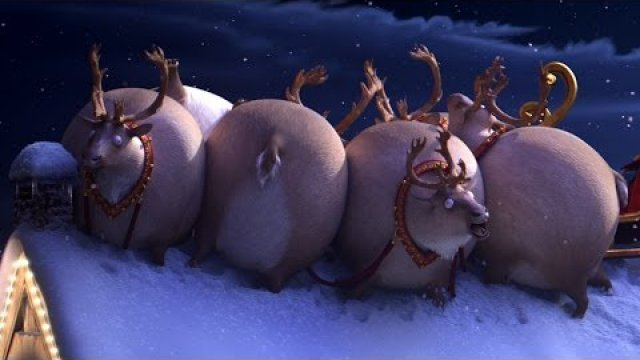
\includegraphics[width=1.00\textwidth]{img/les3-reindeer.jpg}
        \label{fig:les3-reindeer}
      \end{figure}

    \end{column}
  \end{columns}

  Father Christmas wants to fatten his reindeers. Is there an association
  between the amount of proteins in the reindeers' diet and their weight gain?
\end{frame}

\begin{frame}
  \frametitle{Least squares method: example}
  \begin{table}[h] \centering
    \begin{tabular}{@{}rr@{}} \toprule
      Proteins\%& Weight gain (g)  \\
      \midrule
      0   & 177 \\
      10  & 231 \\
      20  & 249 \\
      30  & 348 \\
      40  & 361 \\
      50  & 384 \\
      60  & 404 \\
      \bottomrule
    \end{tabular}
  \end{table}
\end{frame}

\begin{frame}
  \frametitle{Least squares method: example}
  \centering
  \begin{tikzpicture}
    \begin{axis}[
        axis x line=middle,
        axis y line=middle,
        enlarge y limits=true,
        width=\textwidth, height=8cm,     % size of the image
        grid = major,
        grid style={dashed, gray!30},
        ylabel=weight gain (g),
        xlabel=proteins (\%),
        legend style={at={(0.1,-0.1)}, anchor=north}
      ]
      \addplot[only marks] table  {data/santa.txt};
   % \addplot [no markers, thick, red] table [y={create col/linear regression={y=y}}] {data/santa.txt};
    \end{axis}
  \end{tikzpicture}
\end{frame}

\begin{frame}
  \frametitle{Least squares method: example}
  \begin{table}[h] \centering
    \begin{tabular}{@{}llllll@{}}
    	\toprule
    	$x$ & $y$ & $x-\overline{x}$ & $y - \overline{y}$ & $(x-\overline{x})(y - \overline{y})$ & $(x-\overline{x})^{2}$ \\ \midrule
    	0   & 177 & -30              & -130,71            & 3921,3                               & 900                    \\
    	10  & 231 & -20              & -76,71             & 1534,2                               & 400                    \\
    	20  & 249 & -10              & -58,71             & 587,1                                & 100                    \\
    	30  & 348 & 0                & 40,29              & 0                                    & 0                      \\
    	40  & 361 & 10               & 53,29              & 532,9                                & 100                    \\
    	50  & 384 & 20               & 76,29              & 1525,8                               & 400                    \\
    	60  & 404 & 30               & 96,29              & 2888,7                               & 900                    \\
    	    &     &                  &                    & 10990                                & 2800                   \\ \bottomrule
    \end{tabular}
    \caption{Calculations for the least squares method.}
    \label{tab:rendieren2}
  \end{table}
  \[ \beta_{1} = \frac{\sum_{i=1}^{n} (x_{i}-\overline{x})(y_{i} - \overline{y})}{\sum_{i=1}^{n} (x-\overline{x})^{2}} = \frac{10990}{2800} = 3.925 \]
  \[ \beta_{0} = \overline{y} - \beta_{1} \overline{x} = 307.7143 - 3.925 \cdot 30 = 189.96 \]
\end{frame}

\begin{frame}
  \frametitle{Least squares method: example}
  \centering
  \begin{tikzpicture}
    \begin{axis}[
        axis x line=middle,
        axis y line=middle,
        enlarge y limits=true,
        width=\textwidth, height=8cm,     % size of the image
        grid = major,
        grid style={dashed, gray!30},
        ylabel=weight gain (g),
        xlabel=proteins (\%),
        legend style={at={(0.1,-0.1)}, anchor=north}
      ]
      \addplot[only marks] table  {data/santa.txt};
      \addplot [no markers, thick, red] table [y={create col/linear regression={y=y}}] {data/santa.txt};
    \end{axis}
  \end{tikzpicture}
\end{frame}

\section{Correlation coefficient and coefficient of determination}

\sectionframelogo{}

\begin{frame}
  \frametitle{Covariance and correlation}
  \brightbox{\textcolor{HoGentAccent6}{Covariance} is the average deviation of all observations from the mean $(\overline{x}, \overline{y})$.}
  \[\mathrm{Cov}(X,Y) = \frac{1}{n} \sum_{i=1}^{n} (x_i - \overline{x})(y_i - \overline{y})\]
\vfill
  \brightbox{\textcolor{HoGentAccent6}{Pearson's correlation coefficient} ($R$) is a measure for the linear correlation between two variables $X$ and $Y$}
\vfill
  \[R = \frac{\mathrm{Cov}(X,Y)}{\sigma_{X} \cdot \sigma_{Y}} \mathrm{~~~~with~~~~~} -1 \le R \le 1 \]
\vfill  
  \brightbox{The \textcolor{HoGentAccent6}{coefficient of determination} ($R^{2}$) indicates the proportion of the variance in the dependent variable that is predictable from the independent variable(s).}
\end{frame}

\begin{frame}
  \frametitle{Covariance}
  
  Plot of the family size of 15 families in relation to the family size of the mother.
  
  \centering
  \begin{tikzpicture}
    \begin{axis}[
        axis x line=middle,
        axis y line=middle,
        enlarge y limits=true,
        width=\textwidth, height=8cm,     % size of the image
        grid = major,
        grid style={dashed, gray!30},
        ylabel=family size,
        xlabel=family size mother,
        legend style={at={(0.1,-0.1)}, anchor=north}
      ]
      \addplot[only marks] table  {data/families.txt};
      \addplot [no markers, thick, red] table [y={create col/linear regression={y=y}}] {data/families.txt};
    \end{axis}
  \end{tikzpicture}
  We find that $\overline{x} = 3$ and $\overline{y} = 4.3$.
\end{frame}

\tikzset{small dot/.style={fill=black, circle,scale=0.2}}
\tikzset{every pin/.style={draw=black,fill=yellow!10}}

\begin{frame}
  \frametitle{Covariance in the case of linear association}
  \centering
  \begin{tikzpicture}
    \begin{axis}[
        axis x line=middle,
        axis y line=middle,
        enlarge y limits=true,
        width=\textwidth, height=8cm,     % size of the image
        grid = major,
        grid style={dashed, gray!30},
        ylabel=family size,
        xlabel=family size mother,
        legend style={at={(0.1,-0.1)}, anchor=north}
      ]
      \draw (axis cs:3,0)--(axis cs:3,8);
      \draw (axis cs:0,4.3)--(axis cs:6,4.3);
      \node[small dot, pin=120:{$III$}] at (axis cs:1.6,7) {};
      \node[small dot, pin=120:{$I$}] at (axis cs:5.5,7) {};
      \node[small dot, pin=120:{$II$}] at (axis cs:1.6,2) {};
      \node[small dot, pin=120:{$IV$}] at (axis cs:5.5,2) {};
      \addplot[only marks] table  {data/families.txt};
    \end{axis}
  \end{tikzpicture}
\end{frame}

\begin{frame}
  \frametitle{Covariance}
  
  \brightbox{\textcolor{HoGentAccent6}{Covariance} is the average deviation of all observations from the mean $(\overline{x}, \overline{y})$.}
  
  \[\mathrm{Cov}(X,Y) = \frac{1}{n} \sum_{i=1}^{n} (x_i - \overline{x}) (y_i - \overline{y})\]

  Sign of covariance shows \emph{tendency} in the linear relationship between variables
\end{frame}

\begin{frame}
\frametitle{Covariance}

 
  \begin{center}
    \begin{tabular}{cccc}
      Quadrant & $(x_i - \overline{x})$ & $(y_i - \overline{y})$ & $(x_i - \overline{x}) (y_i - \overline{y})$ \\ \hline
      I        & $>0$                   & $>0$                   & $>0$                                        \\
      II       & $<0$                   & $<0$                   & $>0$                                        \\
      III      & $<0$                   & $>0$                   & $<0$ \\
      IV       & $>0$                   & $<0$                   & $<0$ \\
    \end{tabular}
  \end{center}

\begin{itemize}
    \item Cov > 0: increasing/direct relationship
    \item Cov < 0: decreasing/inverse relationship
    \item Cov $\approx$ 0: uncorrelated
  \end{itemize}

\end{frame}

\begin{frame}
  \frametitle{Covariance in the case of randomness}
  \centering
  \begin{tikzpicture}
    \begin{axis}[
        axis x line=middle,
        axis y line=middle,
        enlarge y limits=true,
        width=\textwidth, height=8cm,     % size of the image
        grid = major,
        grid style={dashed, gray!30},
        ylabel=family size,
        xlabel=year of birth mother,
        legend style={at={(0.1,-0.1)}, anchor=north}
      ]
      \draw (axis cs:1942.625,0)--(axis cs:1942.625,6);
      \draw (axis cs:1930,3.4375)--(axis cs:1955,3.4375);
      \node[small dot, pin=120:{$III$}] at (axis cs:1935,5) {};
      \node[small dot, pin=120:{$I$}] at (axis cs:1955,5) {};
      \node[small dot, pin=120:{$II$}] at (axis cs:1935,2) {};
      \node[small dot, pin=120:{$IV$}] at (axis cs:1955,2) {};
      \addplot[only marks] table  {data/families2.txt};
    \end{axis}
  \end{tikzpicture}
  
  We find that $\overline{x} = 1942.625$ and $\overline{y} = 3.4375$; $\mathrm{Cov}(X,Y) = -3.225$
\end{frame}


\begin{frame}
  \frametitle{Pearson's correlation coefficient ($R$)}

  Magnitude of covariance is hard to interpret.\\
  Correlation coefficient (R) is a normalised version of covariance:
\vfill  
  \[R = \frac{\mathrm{Cov}(X,Y)}{\sigma_{X} \cdot \sigma_{Y}} \mathrm{~~~~with~~~~~} -1 \le R \le 1 \]
\vfill  
  R is a number between -1 and 1
\vfill  
  \begin{center}
    \begin{tabular}{rl}
    	$R$ & Interpretation                       \\ \hline
    	-1 & perfect negative linear relationship (decreasing regression line) \\
    	0 & no relationship (horizontal regression line)              \\
    	1 & perfect positive linear relationship (increasing regression line)
    \end{tabular}
  \end{center}

\end{frame}

\begin{frame}
\frametitle{Correlation coefficient}
\begin{figure}
    \centering
    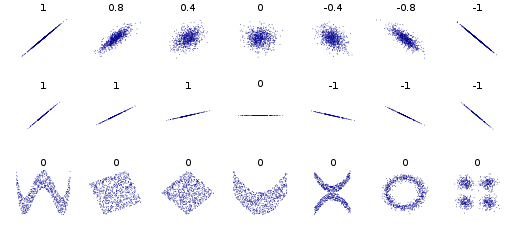
\includegraphics[width=0.90\textwidth]{img/correlationCoef.png}
    \label{fig:les3-regressie}
\end{figure}

\end{frame}

\begin{frame}
\frametitle{Regression line vs. correlation coefficient}
\begin{figure}
    \centering
    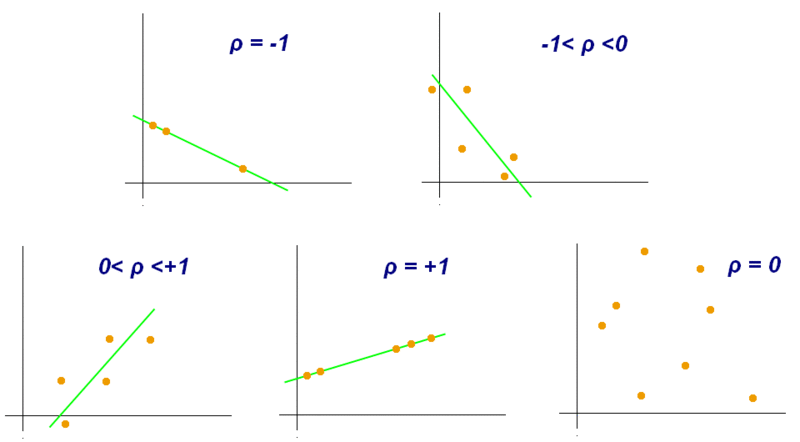
\includegraphics[width=0.90\textwidth]{img/les3-regressie.png}
    \label{fig:les3-regressie}
\end{figure}

\end{frame}


\begin{frame}
  \frametitle{Coefficient of determination ($R^2$)}

  \brightbox{The \textcolor{HoGentAccent6}{coefficient of determination} indicates the proportion of the variance in the dependent variable that is predictable from the independent variable(s).}
  
  \begin{itemize}
    \item If $X$ and $Y$ are unrelated, the best prediction for $y$ is $\overline{y}$
    \item If $X$ and $Y$ are linearly related, the best prediction for $y$ is the regression line $\hat{y} = \beta_0 + \beta_1 \cdot x$
  \end{itemize}
\end{frame}

\begin{frame}
\frametitle{Coefficient of determination ($R^2$)}
  \begin{figure}[t]
    \begin{tikzpicture}
      \begin{axis}[
          axis x line=middle,
          axis y line=middle,
          enlarge y limits=true,
          width=\textwidth, height=8cm,     % size of the image
          grid = major,
          grid style={dashed, gray!30},
          ylabel=weight gain (g),
          xlabel=proteins (\%),
          clip=false,
        ]
        \addplot[only marks] table  {data/santa.txt};
        \addplot [mark=none, color=black] coordinates {
          (0,307.71) (60,307.71)
        };
        \addplot [mark=none, color=blue, thick] coordinates {
          (0,177) (0,307.71)
        };
        \addplot [mark=none, color=blue, thick] coordinates {
          (10,231) (10,307.71)
        };
        \addplot [mark=none, color=blue, thick] coordinates {
          (20,249) (20,307.71)
        };
        \addplot [mark=none, color=blue, thick] coordinates {
          (30,348) (30,307.71)
        };
        \addplot [mark=none, color=blue, thick] coordinates {
          (40,361) (40,307.71)
        };
        \addplot [mark=none, color=blue, thick] coordinates {
          (50,384) (50,307.71)
        };
        \addplot [mark=none, color=blue, thick] coordinates {
          (60,404) (60,307.71)
        };
        \addplot[only marks] coordinates { (20,307.71) };
        \node at (axis cs: 21.3, 316) {$\overline{y}$};
        \node at (axis cs: 21.5, 240) {$y_i$};

      \end{axis}
    \end{tikzpicture}
    \label{fig:rendierenFiguur3}
  \end{figure}
  Total variance $\sigma_{y,total}^2 = \frac{1}{n}\sum (y_i-\overline{y})^2$ = deviation from \textbf{mean} of $y$
\end{frame}

\begin{frame}
\frametitle{Coefficient of determination ($R^2$)}
\begin{figure}[t]
    \begin{tikzpicture}
    \begin{axis}[
    axis x line=middle,
    axis y line=middle,
    enlarge y limits=true,
    width=\textwidth, height=8cm,     % size of the image
    grid = major,
    grid style={dashed, gray!30},
    ylabel=weight gain (g),
    xlabel=proteins (\%),
    legend style={at={(0.1,-0.1)}, anchor=north},
    clip=false,
    ]
    \addplot[only marks] table  {data/santa.txt};
    \addplot [no markers, color=black] table [y={create col/linear regression={y=y}}] {data/santa.txt};
    \addplot [no markers, color=black] coordinates { (0,307.71) (60,307.71) }; % horiz line on mean
    
    \addplot [mark=none, thick, color=red] coordinates { (19.9,249) (19.9,268.4643) };
    \addplot [mark=none, thick, color=green] coordinates { (19.9,307.71) (19.9,268.46) };
    \addplot [mark=none, thick, color=blue] coordinates { (20.1,249) (20.1,307.71) };
    \addplot[only marks] coordinates { (20,307.71) (20,268.46) };
    \node at (axis cs: 21.3, 316) {$\overline{y}$};
    \node at (axis cs: 18.7, 273) {$\hat{y}$};
    \node at (axis cs: 21.5, 240) {$y_i$};
    
    \end{axis}
    \end{tikzpicture}
    \label{fig:rendierenFiguur2}
\end{figure}
  {\color{green}Green}: explained deviation, estimated using linear regression \\
  {\color{red}Red}: unexplained deviation, caused by noise on the data
\end{frame}

\begin{frame}
\frametitle{Coefficient of determination ($R^2$)}
\begin{figure}[t]
    \begin{tikzpicture}
    \begin{axis}[
    axis x line=middle,
    axis y line=middle,
    enlarge y limits=true,
    width=\textwidth, height=8cm,     % size of the image
    grid = major,
    grid style={dashed, gray!30},
    ylabel=weight gain (g),
    xlabel=proteins (\%),
    legend style={at={(0.1,-0.1)}, anchor=north}
    ]
    \addplot[only marks] table  {data/santa.txt};
    \addplot [no markers, color=black] table [y={create col/linear regression={y=y}}] {data/santa.txt};
    \addplot [mark=none, thick, color=red] coordinates {
        (0,177) (0,189.9643)
    };
    \addplot [mark=none, thick, color=red] coordinates {
        (10,231) (10,229.2143)
    };
    \addplot [mark=none, thick, color=red] coordinates {
        (20,249) (20,268.4643)
    };
    \addplot [mark=none, thick, color=red] coordinates {
        (30,348) (30,307.7143)
    };
    \addplot [mark=none, thick, color=red] coordinates {
        (40,361) (40,346.9643)
    };
    \addplot [mark=none, thick, color=red] coordinates {
        (50,384) (50,386.2143)
    };
    \addplot [mark=none, thick, color=red] coordinates {
        (60,404) (60,425.4643)
    };
    
    \end{axis}
    \end{tikzpicture}
    \label{fig:rendierenFiguur2}
\end{figure}
Unexplained variance $\sigma_{y,unexpl}^2 = \frac{1}{n}\sum (y-\hat{y})^2$ = deviation from \textbf{estimate} for $y$ based on regression line
\end{frame}

\begin{frame}
\frametitle{Coefficient of determination ($R^2$)}

Let

\[ \sigma_{y,total}^2 = \frac{1}{n} \sum_{i=1}^{n} (y_i - \overline{y})^2 \textrm{ (total sample variance)}\]
\[ \sigma_{y,unexpl}^2 = \frac{1}{n} \sum_{i=1}^{n} (y_i - \hat{y})^2 \textrm{ (unexplained variance)}\]

\begin{itemize}
  \item If $x$ doesn't contribute to $y$, then $\sigma_{y,unexpl}^2 \approx \sigma_{y,total}^2$
  \item If $x$ does contribute to $y$, then $\sigma_{y,unexpl}^2 < \sigma_{y,total}^2$
\end{itemize}

\[R^2 = \frac{\sigma_{y,total}^2 - \sigma_{y,unexpl}^2}{\sigma_{y,total}^2} = \frac{\textrm{explained variance}}{\textrm{total sample variance}}\]

\end{frame}

\begin{frame}
  \frametitle{Correlation coefficient and coefficient of determination}
  \begin{table}[h] \centering
    \begin{tabular}{@{}|r|r|r|r|@{}}
    	\toprule
    	          $R$ &       $R^{2}$ & Explained variance &   Interpretation \\ \midrule
    	      $< 0,3$ &       $< 0,1$ &           $< 10\%$ &        very weak \\
    	  $0,3 - 0,5$ & $0,1 - 0,25$ &        $10 - 25\%$ &             weak \\
    	  $0,5 - 0,7$ &  $0,25 - 0,5$ &        $25 - 50\%$ &          average \\
    	 $0,7 - 0,85$ &  $0,5 - 0,75$ &        $50 - 75\%$ &           strong \\
    	$0,85 - 0,95$ &  $0,75 - 0,9$ &        $75 - 90\%$ &      very strong \\
    	     $> 0,95$ &       $> 0,9$ &            $>90\%$ & exceptional(!) \\ \bottomrule
    \end{tabular}
  \end{table}

\end{frame}

\begin{frame}
  \frametitle{Application (reindeers)}
  \begin{columns}
    \begin{column}{0.5\textwidth}
      \begin{table}[h] \centering
        \begin{tabular}{@{}rrr@{}} \toprule
          $(x-\overline{x})$ & $(y - \overline{y})$ & $(x-\overline{x})(y - \overline{y})$ \\
          \midrule
          $-30$ & $-130.714$ & $3921.429$ \\
          $-20$ & $-76.7143$ & $1534.286$ \\
          $-10$ & $-58.7143$ & $587.1429$\\
          $0$   & $40.28571$ & $0$\\
          $10$  & $53.28571$ & $532.8571$\\
          $20$  & $76.28571$ & $1525.714$\\
          $30$  & $96.28571$ & $2888.571$\\
          \bottomrule
        \end{tabular}
      \end{table}
    \end{column}
    \begin{column}{0.5\textwidth}
      \[ \sum_{i}^{n} (x-\overline{x})(y - \overline{y}) = 10990 \]
      \[ Cov = \frac{10990}{7} = 1570 \]
      \[ \sigma_{x} = 20 \]
      \[ \sigma_{y} = 81.03 \]
      \[ R = \frac{1570}{20 \cdot 81.03} = 0.96 \]
      \[ R^{2} = 0.93 \]
    \end{column}
  \end{columns}
\end{frame}

\begin{frame}
  \frametitle{Considerations}
  
  \begin{itemize}
    \item The correlation coefficient only measures the association between \emph{two} variables. Interactions with other variables are not considered.
    \item The correlation coefficient only expresses \emph{linear} associations.
    \item Correlation does not imply causation!
  \end{itemize}
\end{frame}

\begin{frame}
\frametitle{functions in R}

\begin{itemize}
    \item \texttt{lm()} (linear model): generates $\beta_0$ and $\beta_1$
    \item \texttt{cov()}: generates the covariance value
    \item \texttt{cor()}: generates the (Pearson's) correlation coefficient R
\end{itemize}
\end{frame}

%---------- Back matter -------------------------------------------------------

\end{document}
